\section{評価}
\label{sec:evaluation}
\subsection{プロトタイプ実装とシミュレーション環境}
\label{sec:simulation}
%ここではプロトタイプ実装とネットワーク環境を説明すればいい
提案システムにおけるトンネリング抑止機能の評価にあたり,システムのプロトタイプをPython3を用いて実装した.
実装では,DNSパケットの作成およびパース(分解)のためにdnslibライブラリを使用した.
また,マネージャにおけるコンテンツ管理には,Redisデータベースを使用した.
フルサービスリゾルバとマネージャのサービスを実装し,Dockerに基づいた仮想環境上でコンテナをサービスノードとして動作させることによる擬似的な名前解決基盤を構築した.
スタブリゾルバから,名前解決のクエリとしてdigコマンドを使用した.
%表~\ref{tab:software_version}に,使用したソフトウェアとそのバージョンを示す.
%\begin{table}[b]
 \caption{使用したライブラリと環境}
 \centering
  \begin{tabular}{lrr}
    \toprule
		\multicolumn{1}{c}{\textbf{ソフトウェア}} & \multicolumn{1}{c}{\textbf{バージョン}} \\
    \midrule
    Python & 3.7.5 \\
    Docker & 19.03.5 \\
    dnslib & 0.9.10 \\
    Redis & 3.3.11 \\
		dig & 9.10.6\\
    \bottomrule
  \end{tabular}
 \label{tab:software_version}
\end{table}

%なぜRedisなのか
%提案システムにおいて,データ管理として求められる要件は,コンテンツの永続性である.

次に,Docker環境上に構成したネットワーク構成について説明する.
ネットワークは,一般的な組織内からインターネットに設置されている外部リソースにアクセスするために,インターネット上に設置されたサーバ(マネージャ)にアクセスするというシナリオに基づいて設計した.
また,組織におけるインターネット利用は,インターネットに設置されたオープンリゾルバや直接サーバに接続することを防止するためにOP53Bが設定されているという想定である.
そのため,図~\ref{fig:exp-network-topology}で示すように,組織内部のスタブリゾルバは同内部のフルサービスリゾルバを経由して,インターネット上のマネージャに問い合わせられることで名前が解決される.

\begin{figure}[htbp]
 \centering
 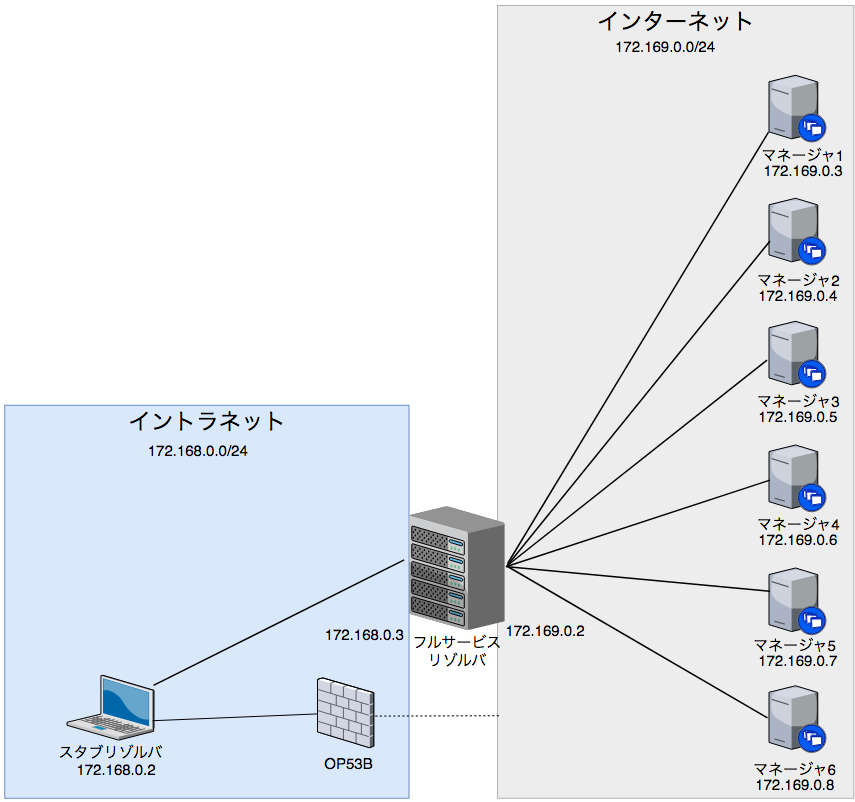
\includegraphics[scale=0.2]{figure/exp-network-topology.png}
 \caption[実験に用いたネットワークトポロジー]{Docker環境内におけるネットワークトポロジー}
 \label{fig:exp-network-topology}
\end{figure}

%\newpage
\subsection{DNSトンネリング}
\label{sec:eval-tunnel}
%目的が見えない
%本節では,提案システムのDNS Exilfiltration抑止機能について,擬似DNSトンネリングの通信を提案システム上で発生させるシミュレーションに基づいて評価した結果を示す.
シナリオは,DNS Exiltrationの手法に基づいて,スタブリゾルバから``exfil.com"を宛先にDNSクエリが発せられることを想定する.
DNSトンネリングの問い合わせに用いる擬似ドメイン名には,1文字から63文字の長さでランダムな文字列で生成されたラベルを5000個を用意し,ドメインが``exil.com"となるようにそのラベルをホスト名として組み合わせたドメイン名を作成した.
DNS Exfiltrationでは,問い合わせるリソースレコードのタイプの種類は関係ないため,全てAレコードを設定した.
実験では,先の5000個のドメイン名を問い合わせるスクリプトを用意し,スタブリゾルバからクエリさせた.
クエリは既存システム同様,はじめに組織内部のフルサービスリゾルバに転送される.
フルサービスリゾルバは,問い合わせられたドメイン名とレコードタイプからドメインIDとコンテンツIDを算出し,コンテンツを保持するマネージャのアドレスをコンテンツIDに基づいて決定する.
QuestionセクションのQnameには,識別子である``コンテンツID.ドメインID"が含まれている.
このような仕組みによって,スタブリゾルバからのクエリは,コンテンツを操作するプロバイダを介在せずに名前解決を行える.
このメカニズムによって,任意のサーバをデータ転送先とするDNS Exfiltrationの発生を抑止する.
\subsection{特性評価}
\subsubsection{トラフィック量}
%クエリMinimisationがどの程度普及しているのかによって,計算方法が随分と異なることが予想される
%Query Minimisationの場合は,どのようになるのか
本項では,名前解決に伴って発生するトラフィック量を比較評価した結果を示す.
%表~\ref{tab:diff_dns-td_dns}で示すように,提案システムではサーバへの問い合わせは一回で済む.
既存システムでは,コンテンツを保持するサーバまで再帰的に問い合わせることを踏まえると,提案手法の方がトラフィック数は少なくなる.
一方で,既存システムは任意のドメイン名が使用されるのに対して,提案システムでは常に固定長の85bytesのドメイン名が使用される.

トラフィック量の評価においては,クエリパケットのみに焦点を当てた.
既存システムにおける再帰問い合わせでは,ルートからTLD,SLDと権威サーバのアドレスがAuthoirityセクションに含まれて応答されるが,問い合わせられるドメイン名ごとで委譲されている数が異なる.
また,権威サーバのアドレスとして含めることができるアドレスは一つでないため,応答パケットのサイズにはドメイン毎にランダムである特性がある.
このように応答パケットのサイズはドメイン依存であるため推定することが困難である.
以上から,トラフィック量の推定には,クエリパケットのみを焦点に当てた.
また,既存システムと提案システムのスタブリゾルバからフルサービスリゾルバまでの通信は両者とも共通であるため,評価するトラフィックはフルサービスリゾルバとサーバ(権威サーバ,マネージャ)間の通信を評価した.
評価では,長さの異なる253種類のドメイン名をスタブリゾルバからクエリし,フルサービスリゾルバから権威サーバまでのクエリパケットのサイズを対象とした.
既存システムでは,権威サーバへの問い合わせる方法には,2つの種類がある.
1つ目は,通常の全ての権威サーバに同じFQDNで問い合わせる方法である.
この場合,権威サーバを宛先とするパケットは,常に同じパケットサイズとなる.
2つ目は,宛先となる権威サーバにはその次の権威サーバのドメイン名のみを問い合わせるQname Minimisation~\cite{rfc7816}と呼ばれる手法である.
Qname Minimisationは,権威サーバに問い合わせるQuestionセクションのドメイン名が最小限に留められる.
例えば,``www.example.com"について考える.
フルサービスリゾルバにおいてQname Minimisationの設定が有効になっている場合,ルート権威サーバには``com"のNSレコード情報が問い合わせられる.
同様にして,``com"権威サーバには,``example.com"のNSレコード情報が問い合わせられるという具合である.

はじめに,ルートのAレコードタイプに関するクエリパケットのサイズを収集した.
次に,全てのTLDのドメイン名を収集し,TLDのAレコードタイプに関するクエリパケットのサイズを収集した.
また,全てのドメインの長さパターンにおけるパケットサイズのデータを収集した.
Qname Minimisationを使用しない場合,名前解決に伴うクエリの総トラフィックサイズは,以下の計算式で求めることができる.\\

(n\ Label's\ Traffic) \\
 $= (R + (Label\ Length) + r + Rtype + O) \times n$\\
 $= (1 + (Label\ Length) + 1 + 1 + 68) \times n$\\
 $= (71 + (Label\ Length)) \times n$\\
\begin{table}[h]
 \caption{パケット構成する要素とそのサイズ}
 \centering
  \begin{tabular}{llr}
    \toprule
		\multicolumn{1}{c}{\textbf{表記}} & \multicolumn{1}{c}{\textbf{意味}} & \multicolumn{1}{c}{\textbf{サイズ(bytes)}} \\
    \midrule
		R & ラベルの長さを示す領域 &  \begin{tabular}{r}1\end{tabular} \\
		r & Rootを表す``."をストアする領域 & \begin{tabular}{r}1\end{tabular} \\
		O & Qname以外のクエリパケットサイズ & \begin{tabular}{r}68\end{tabular} \\
		Rtype & レコードタイプ & \begin{tabular}{r}1(A)\\2(NS)\end{tabular}\\
    \bottomrule
  \end{tabular}
 \label{tab:root-tld-packet-size}
\end{table}


図~\ref{fig:length-size}は,DNSとDNS-TDにおける名前解決で発生するクエリパケットの総トラフィック量の比較結果である.
x軸がスタブリゾルバから問い合わせられたドメイン名の長さで,y軸が総トラフィック量である.

\begin{figure}[htbp]
 \centering
 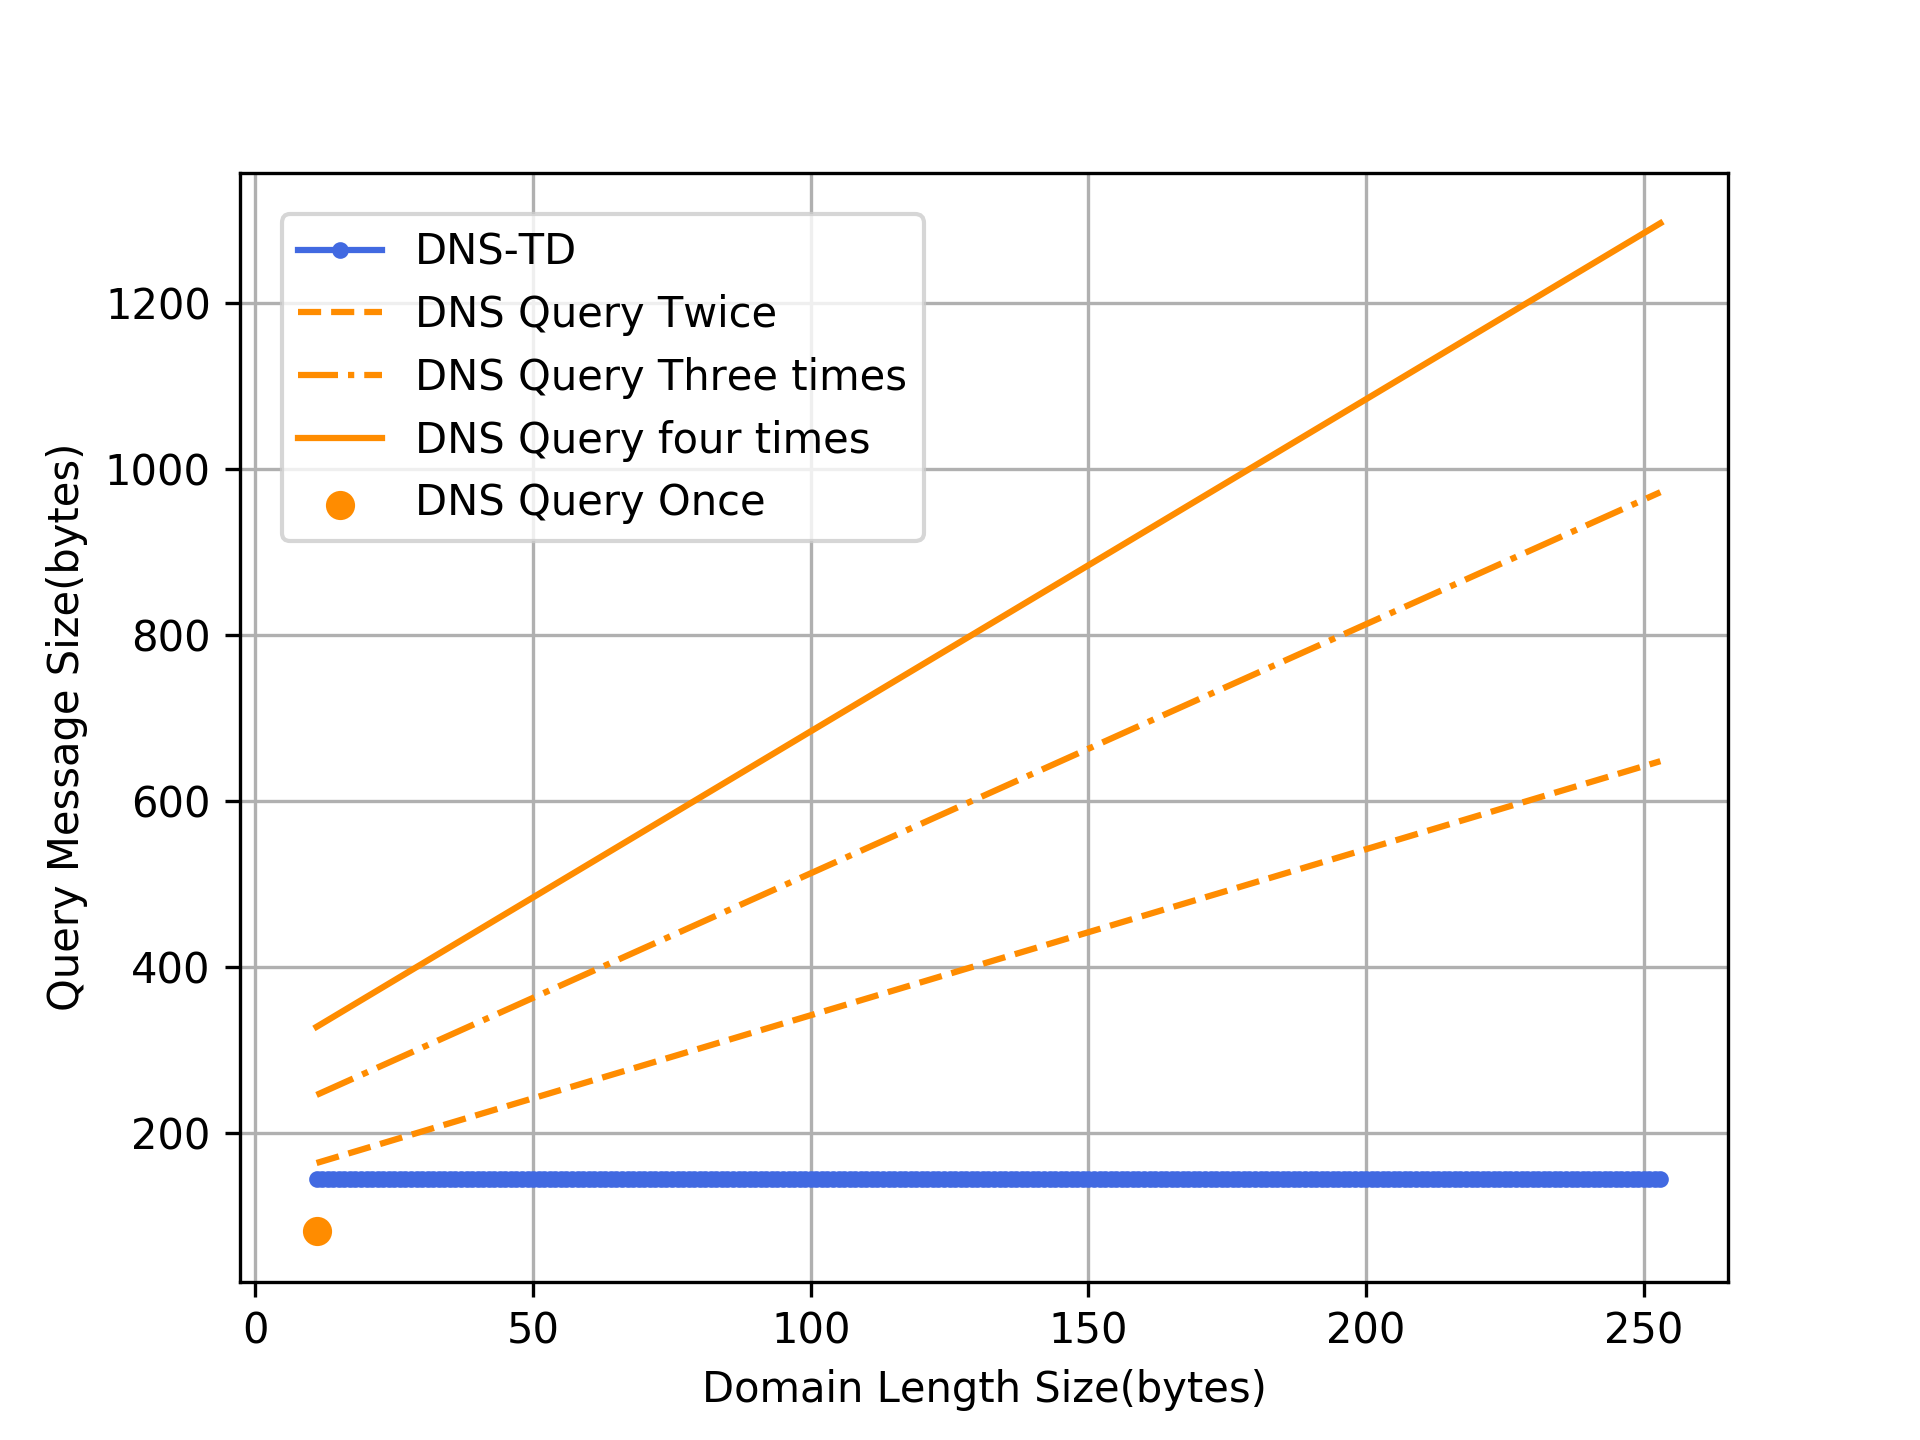
\includegraphics[scale=0.4]{figure/length-size.png}
 \caption[DNSと提案システムのクエリパケットサイズ比較]{DNS-TDとDNSにおける名前解決に使用されるクエリパケットサイズの比較}
 \label{fig:length-size}
\end{figure}

%  9: 243bytes
% 10: 246bytes

図~\ref{fig:length-size}から,Qname Minimisationを使用しない場合では,提案システムのような固定長の方が再帰的に問い合わせるよりもトラフィック量は抑えられることが確認できる.

%次に,Qname Minimisationが適用されている場合を考える.
%Qname Minimisationを使用する場合,名前解決時に必要となるそうトラフィックサイズは,以下の計算式から求めることができる.
%\begin{eqnarray}
% (n\ Label's\ Traffic) &=& (R + (Label\ Length) + r + O) \times n\\
% &=& (1 + (label\ Length) + 1 + 69) \times n\\
% &=& 71 \times (Label\ Length) \times n
%\end{eqnarray}
%

%以上の検証結果より,提案システムの方が既存システムと比べてクエリトラフィック量を抑えられることが確認できた.
%DNS-TDでは,シンボル志向の名前解決メソッドによって,既存の再帰問い合わせによるメソッドよりも少ないトラフィックに抑えることが期待される.

%\newpage
\subsubsection{オーバーヘッド}
%提案システムにおいて,マネージャの機能は既存システムにおけるTLDの権威サーバが担当することを想定している.
%このため,提案システムでは,マネージャまでのトラフィック
%ハッシュ計算に伴うオーバーヘッドについて
提案システムの名前解決メカニズムでは,名前解決問い合わせの都度,コンテンツIDとドメインIDを導出する必要がある.
ハッシュ関数に基づいているこの2つの識別子を導出する処理は,名前解決処理におけるオーバーヘッドになることが予想される.
本項では,識別子の導出処理に伴う時間的なオーバーヘッドについて,検証実験に基づいて評価した結果を示す.

評価では,はじめに``exfil.com"をドメインとするランダムに作成した5000個のホスト名とリソースレコードのタイプの組を用意した.
その組からコンテンツIDとドメインIDを導出するのにかかった時間の計測した.
この操作を4回繰り返し,組ごとのダイジェスト導出にかかった時間の平均をとったのが,表~\ref{fig:overhead}である.
処理時間を計測には,Python3における精度評価に用いられるtimeライブラリのperf\_counterメソッドを用いた.
検証環境は,表~\ref{tab:overhead-test}の通りである.

\begin{table}[h]
 \caption{識別子算出のパフォーマンステスト環境}
 \centering
  \begin{tabular}{lr}
    \toprule
		\multicolumn{1}{c}{\textbf{要素}} & \multicolumn{1}{c}{\textbf{環境}} \\
    \midrule
		OS & MacOS(10.14.6) \\
		CPU & 1.6GHz\ Intel\ Core\ i5 \\
		メモリ & 8GB\ 1600GHz\ DDR3 \\
    \bottomrule
  \end{tabular}
 \label{tab:overhead-test}
\end{table}


図~\ref{fig:overhead}で示す検証の結果から,識別子の組を導出するのにかかる時間は約0.003ミリ秒の分布する.
名前解決にかかる時間は,ルート権威サーバを例にとると図~\ref{fig:root-rtt}で示すように,0から1000ミリ秒と振り幅はあるものの明らかに識別子にかかる時間は無視できる程度に小さいことが確認できる.
以上から,提案システムにおける識別子導出にかかる時間的オーバーヘッドは無視できるものと捉えられる.

\begin{figure}[htbp]
 \centering
 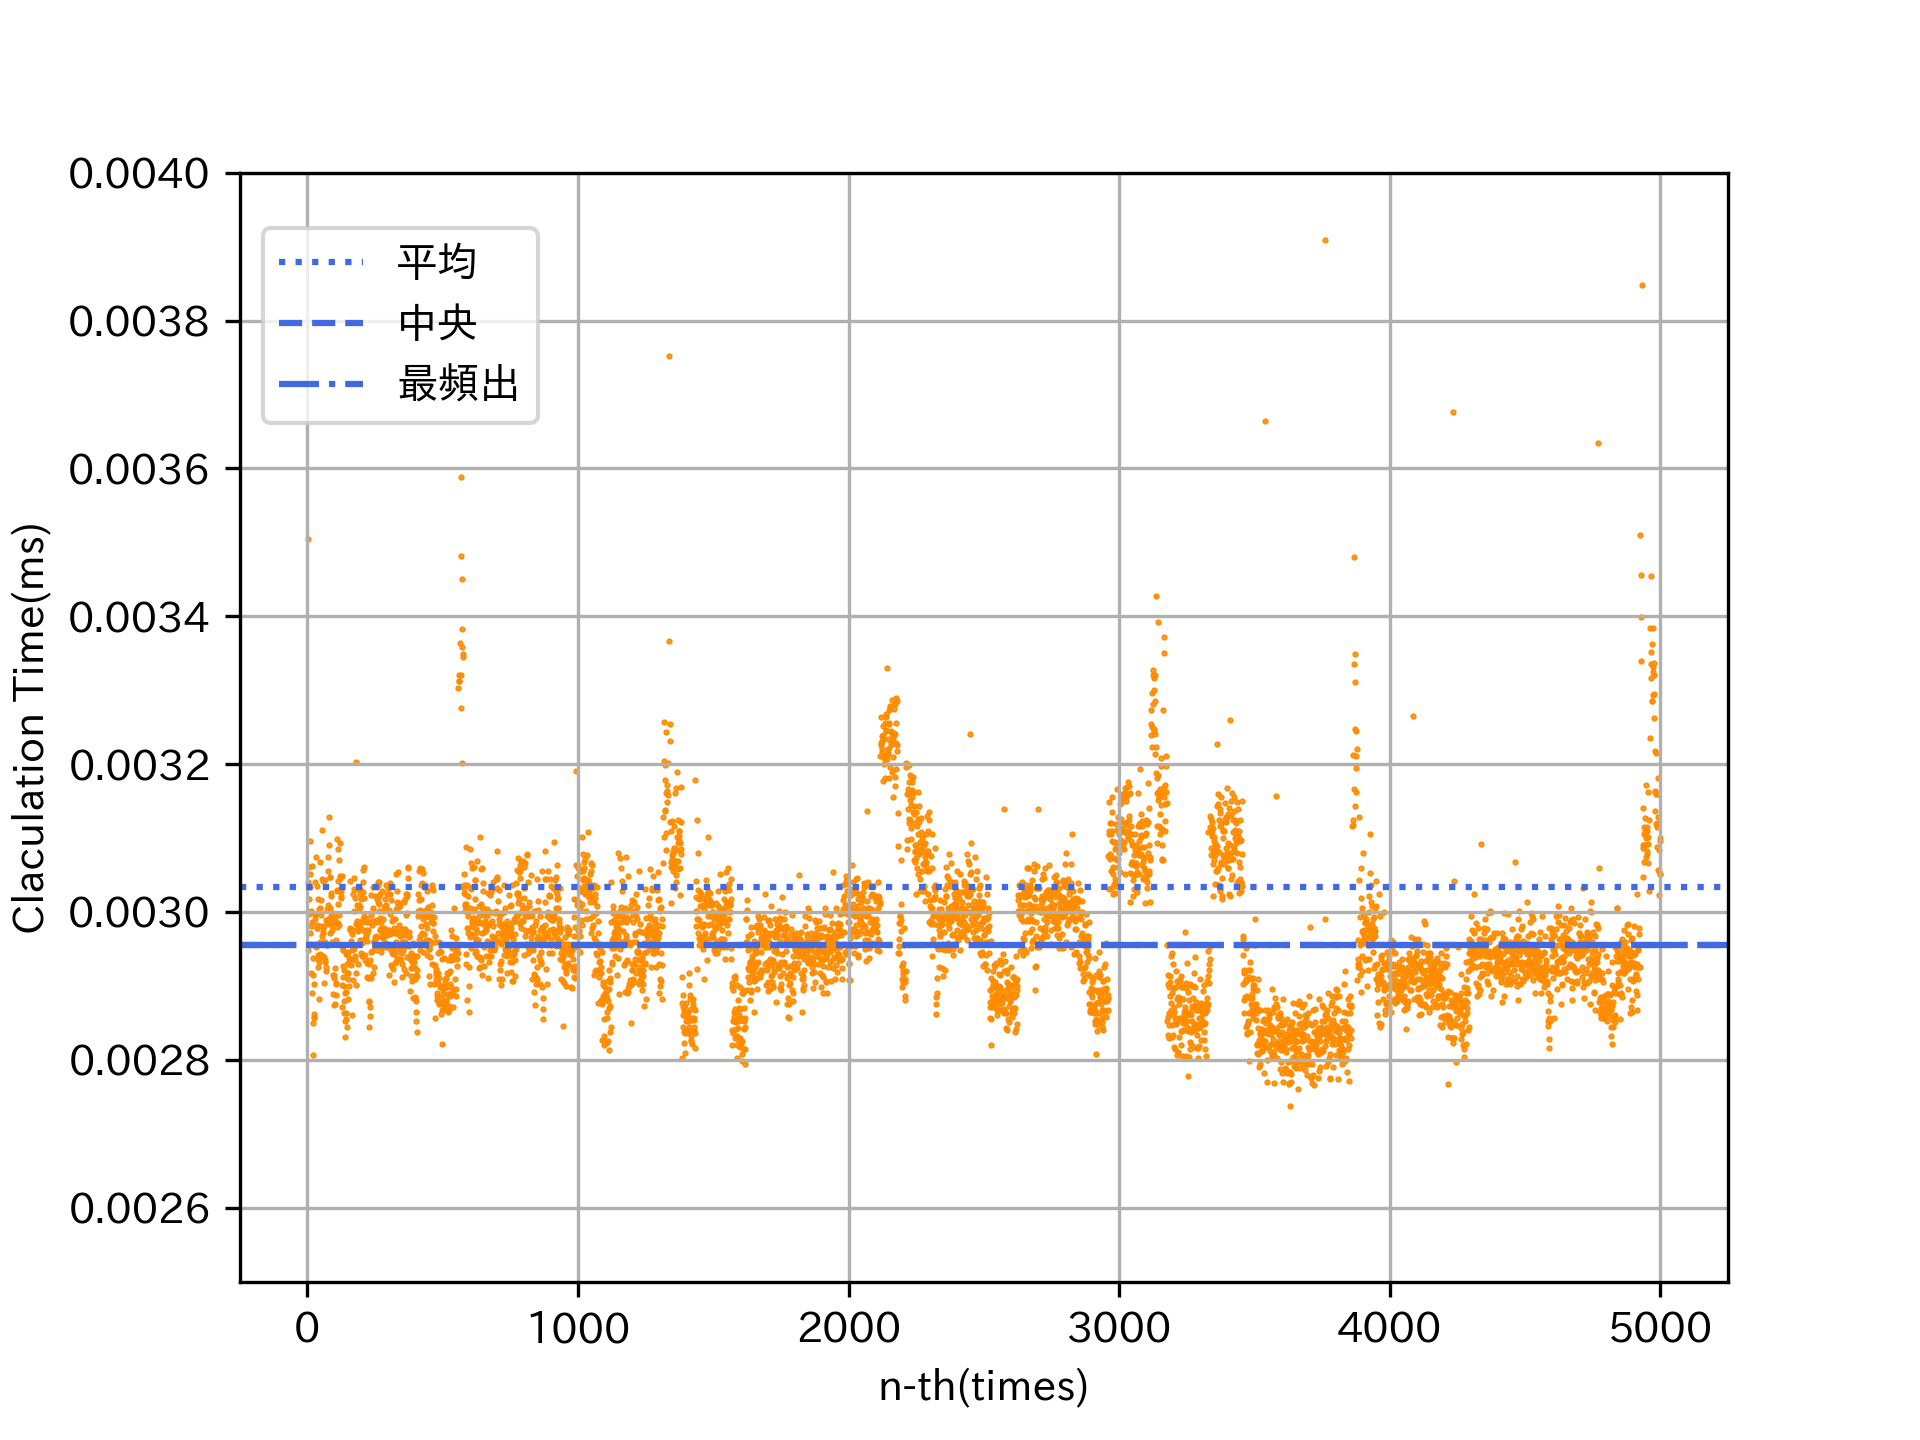
\includegraphics[scale=0.4]{figure/overhead.png}
 \caption[識別子導出にかかる時間的オーバーヘッド]{コンテンツIDとドメインID導出にかかる計算時間のオーバーヘッド}
 \label{fig:overhead}
\end{figure}
%処理にかかるメモリのオーバーヘッドについて


%DNSは,現在のインターネットの根幹に位置する技術であるため,DNSトラフィックはインターネット全体に大きく影響する.
%\newpage
\subsubsection{名前解決速度}
\label{sec:resolution_speed}
提案システムでは,コンテンツを保持するサーバはコンテンツIDから一意に定まる.
一方,既存システムでは,ルートから階層的にコンテンツを保持するサーバを探索した後に定まるため,提案システムの方が高速に名前解決できることが期待される.
この特性を踏まえて,本項では,既存システムとの秘匿に基づいて名前解決速度について評価する.

名前解決速度の評価には,フルサービスリゾルバによる問い合わせに対する権威サーバからの応答までの時間に基づいて評価する.
提案システムにおいて,マネージャサービスは既存システムにおけるTLDが担当する.
% キャッシュを前提とすると速度の期待値はそこまで高くないかも
% 既存のDNSにおけるラウンドトリップのうち,再帰問い合わせの最後の権威サーバRTTがdns-tdのフルリゾルバとマネージャのそれになる.
% 遠いものと近いもののRTTを用意する必要がある
図~\ref{fig:root-rtt}で示すように,ルート権威サーバまでのRTTは50ミリ秒周辺が最も多く,平均すると100ミリ秒に収束する.
他方で,図~\ref{fig:tld-rtt}で示すように,TLD権威サーバまでのRTTは13ミリ秒周辺が最も多く,平均は50ミリ秒に収束することがわかる.
既存システムでは,問い合わせるドメイン名のゾーン構成に従い,最終的な権威サーバまでのRTTが加算される.
他方で,提案システムでは,TLDを想定するマネージャにフルサービスリゾルバから1ホップの問い合わせで名前解決が実現される.
以上のことから,少なくてもSLD以降の権威サーバにかかるRTT分高速に名前解決できることがわかる.
\begin{figure}[htbp]
 \centering
 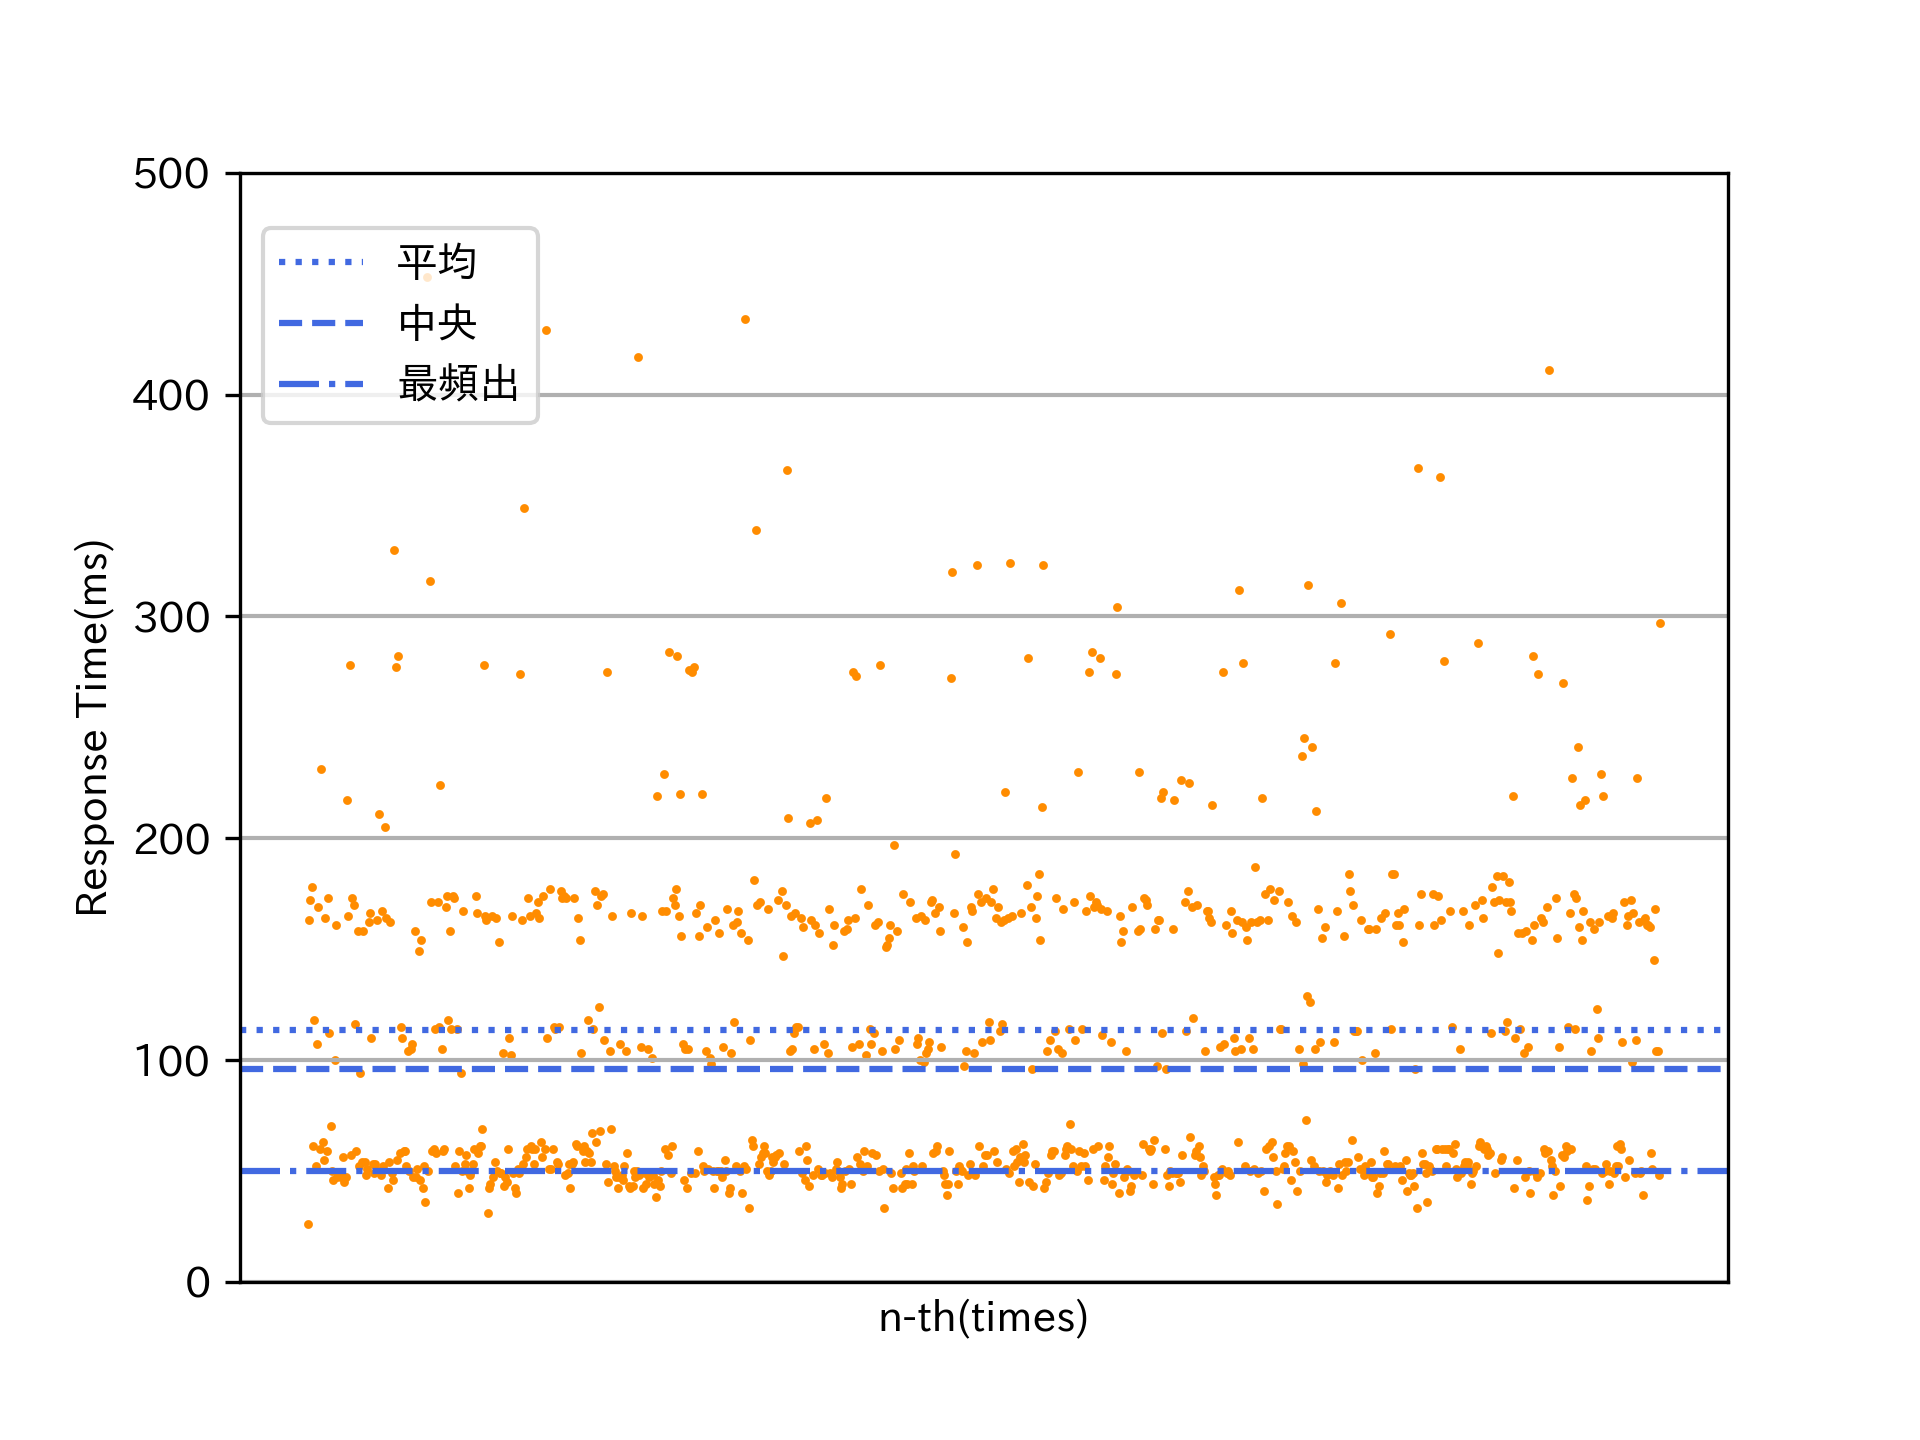
\includegraphics[scale=0.4]{figure/root-rtt.png}
 \vspace{-0.5cm}
 \caption{Root権威サーバにおけるRTTの分布}
 \label{fig:root-rtt}
 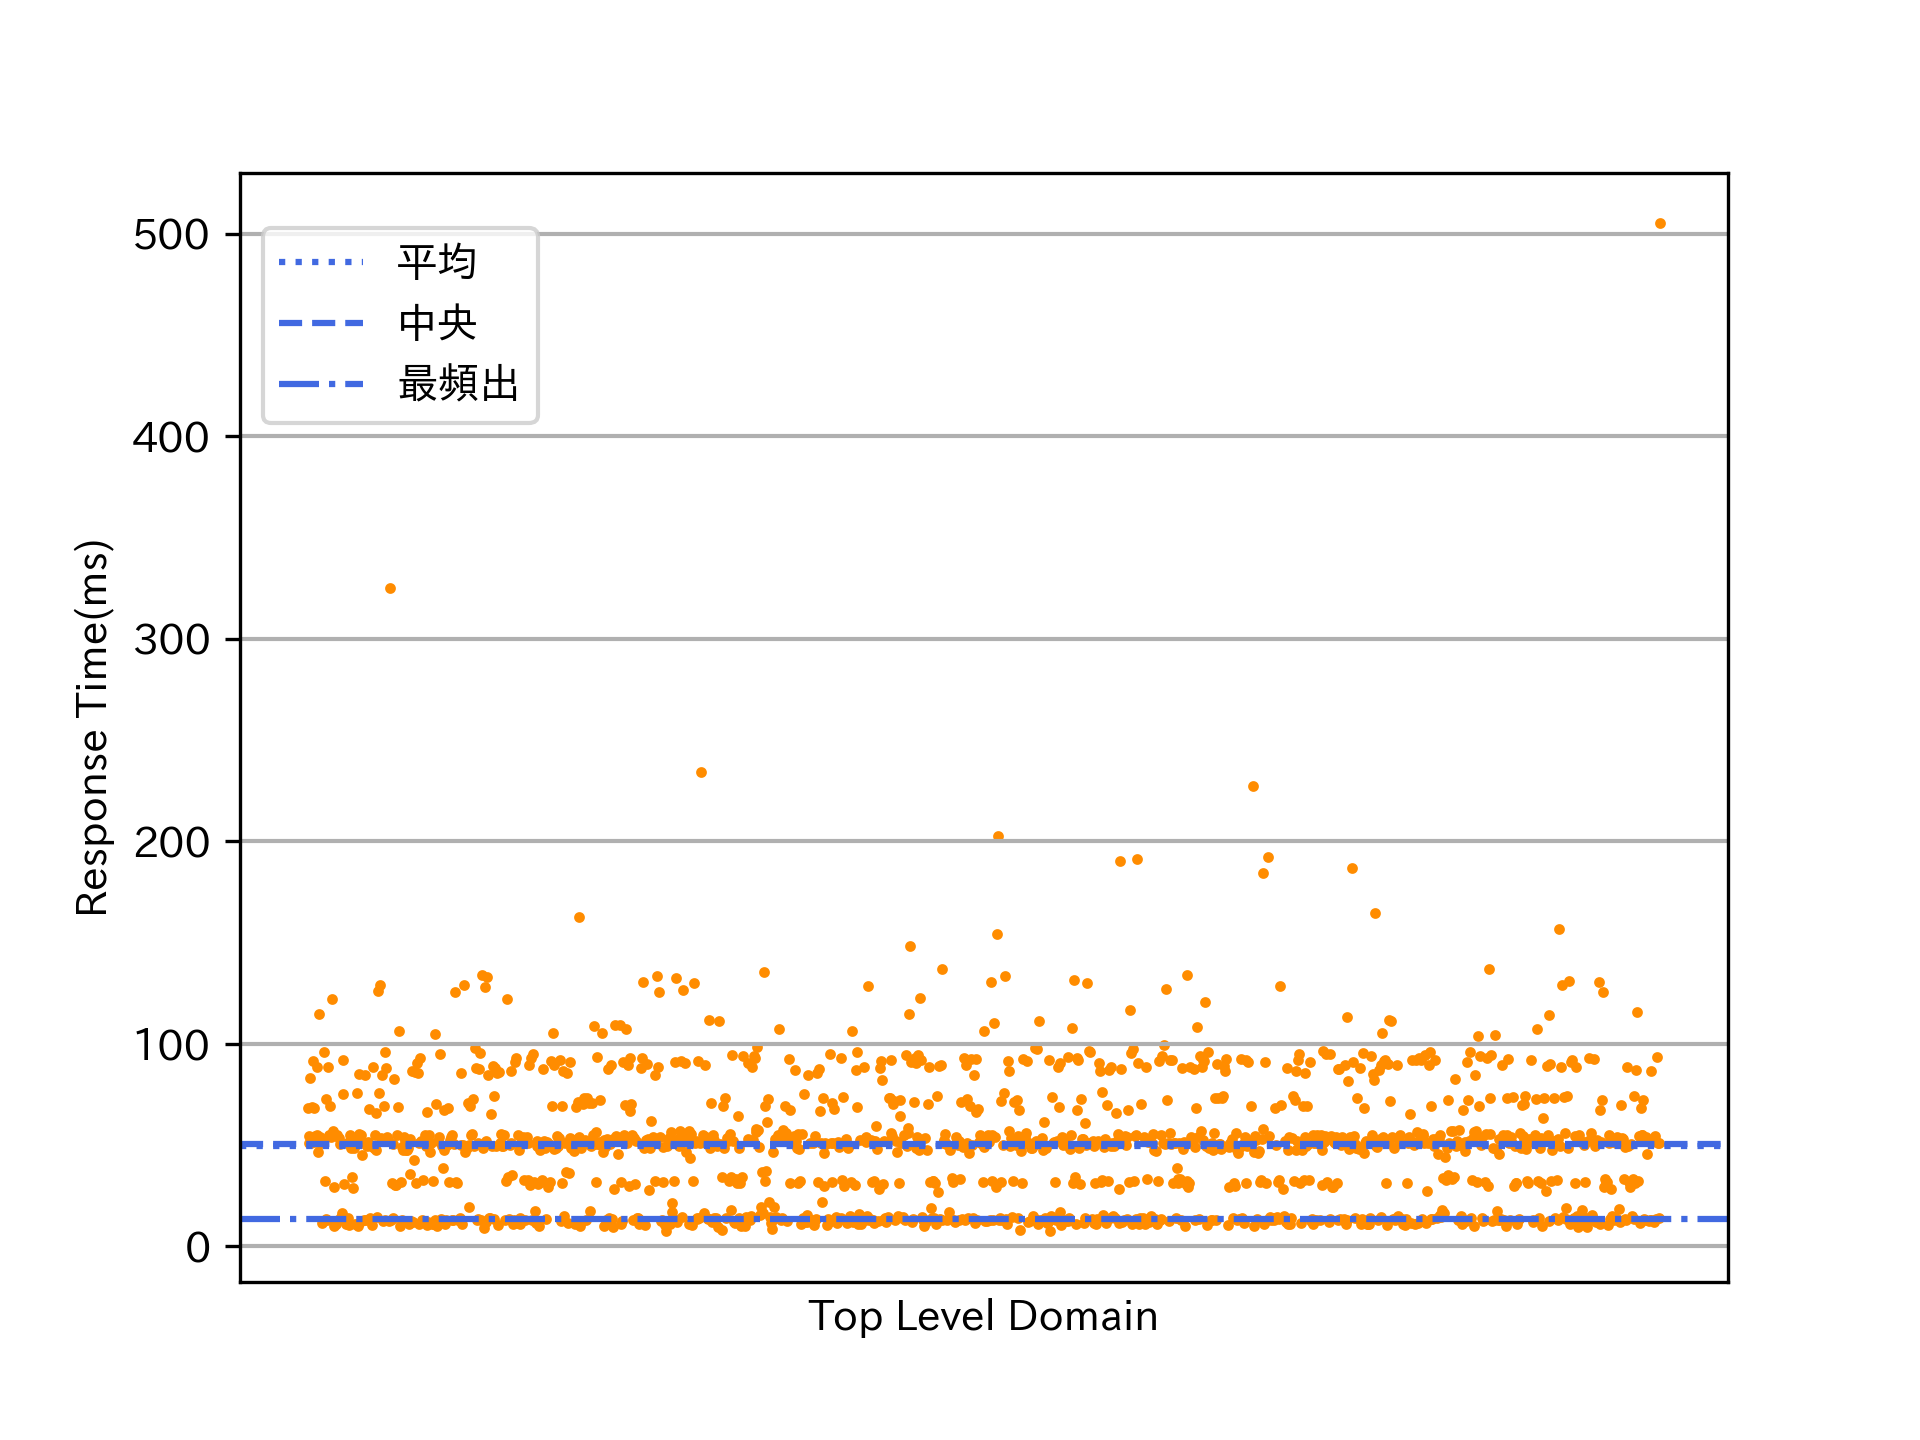
\includegraphics[scale=0.4]{figure/average_rtt.png}
 \vspace{-0.5cm}
 \caption{TLD権威サーバにおけるRTTの分布}
 \label{fig:tld-rtt}
\end{figure}

%\subsubsection{要件に基づく評価}
%最後に,次世代ネットワークとして提案されているICN(Information-Centric Networking)\footnote{ICN : サーバ指向のネットワーキングではなくコンテンツ指向のネットワーキング.}の名前解決システムの要件として議論されているインターネットドラフトを用いて評価を行った~\cite{irtf-icnrg-nrs-requirements-03}.
%当該要件は,一つ目の``ICNにおける名前解決機能"は明らかにICN固有の要素であるのに対して,その他のガイドラインとセキュリティに関する事柄は,名前解決システムの要件として一般化できる内容であると考えられる.
%以降で示す要件は,ICNにおける名前解決システムの要件を翻訳したものである.
%%本研究では,さらに名前解決に伴うトラフィック量についても評価の項目に含めた.
%
%\begin{description}
% \item[ICNにおける名前解決機能]\mbox{}\\
%	 \vspace{-9mm}
%	\begin{enumerate}
%   \item スケーラブルなルーティングシステムのサポート
%	 \vspace{-3mm}
%	 \item オフパスキャッシュ機能のサポート
%	 \vspace{-3mm}
%	 \item 名前なしオブジェクトのサポート
%	 \vspace{-3mm}
%	 \item マニフェストのサポート
%	 \vspace{-3mm}
%	 \item メタデータのサポート
%	\end{enumerate}
% \item[ICNにおける名前解決の設計ガイドライン]\mbox{}\\
%	 \vspace{-9mm}
%	\begin{enumerate}
%	\item 名前解決速度
%	 \vspace{-3mm}
%	\item 応答の正確性
%	 \vspace{-3mm}
%	\item 名前解決の保証
%	 \vspace{-3mm}
%	\item 公平な名前解決
%	 \vspace{-3mm}
%	\item スケーラビリティ
%	 \vspace{-3mm}
%	\item 管理のし易さ
%	 \vspace{-3mm}
%	\item 配備されたシステム
%	 \vspace{-3mm}
%	\item 故障耐性
%  \end{enumerate}
% \item[セキュリティに関する事柄]\mbox{}\\
%	 \vspace{-9mm}
%	\begin{enumerate}
%   \item 可用性
%	 \vspace{-3mm}
%	 \item 認証
%	 \vspace{-3mm}
%	 \item データの機密性
%	 \vspace{-3mm}
%	 \item プライバシーの保護
%	 \vspace{-3mm}
%	 \item ロバストネス・レジリエンス
%	 \vspace{-3mm}
%	 \item ネットワークプライバシー
%	\end{enumerate}
%\end{description}

%\subsubsection{評価項目に基づいた特性の評価}

% DDoSへの影響については,リクエストとレスポンスパケットのサイズからアンプ率に着目する
%DNS-TDでは,56byteを固定長とするコンテンツIDをシンボルとすることによって,レコード情報にアクセスする.
%この仕組みの影響で,DNS-TDのパケットは従来のパケットと比較して肥大する特性がある.
%このため,送信元を目的ホストと偽装することで目的ホストの計算リソースを圧迫するDDoS攻撃に対して,脅威を高める可能性が予想される.

% 比較項目
% 従来のドメインごとにゾーンが分離している設計と違い,一つのゾーンには様々な組織のドメインが管理されている.
% アンプ率は,既存のDNSと基本的に変わらない.DNSSECがあるかないかについて議論するくらい
